\chapter{Fundamental Concepts}
\fett{TODO: In this chapter we...}
This chapter lays out the fundamental concepts that are needed in order to discuss the topic.
Subchapter 2.1 presents and elucidates the basic concept of stream processing, afterwards
subchapter 2.2 defined self-adaptive systems and explains their core features.
\section{Stream Processing}
Note (Will be removed): This subchapter should explain why stream processing is needed, when it is applied, how it works
\subsection{Stream Processing Systems}
\fett{TODO: Wie sieht Data in SPS aus? discuss with DBMS approach, too}
\subsection{Data Stream Management Systems}
vergleichen mit dbms blabla
\subsection{Requirements for Stream Processing Systems}
\fett{HIER NOCH DIE EINZELNEN PUNKTE ELABORATEN WIESO DIESE WICHTIG FÜR UNS SIND}
Due to the nature of the fields in which SPS are used, there are important requirements that SPS should meet in order to be viable, which Stonebraker et al. point out in [SOURCE], which can be summarized as the following:
\begin{enumerate}
\item \fett{Keep the Data Moving:} In order to minimize latency, data must not be stored, as these are costly operations.
\item \fett{Handle Stream Imperfections:} Expecting only perfect data is utopian, so one must prepare the system with built-in mechanisms for data that might be missing or out-of-order.
\item \fett{Integrate Stored and Streaming Data:} For an SPS to be able to perform comparisons between "predecessor" data and current data, operators must keep an efficiently manageable state.
\item \fett{Guarantee Data Safety and Availability:} Recovering from a failure is detrimental for real-time data processing, so a system must be in place to guarantee the highest availability possible.
\item \fett{Process and Respond Instantaneously:} Systems must be highly optimized in order to provide (near) real-time responses.
\end{enumerate}
An SPS takes in one or multiple continuous streams of data, each element of the stream then gets processed by a number of operators and eventually, the SPS puts out a stream of processed data.

In order to increase efficiency, an SPS can, if (computational) resources are available, create replicas of operators to introduce parallelity. Conversely, if there is little input, it may also reduce the amount of replicas in order to save or free up additional resources.
\textit{Figure 2.3 should be here}
\begin{figure}[htb]
\centering
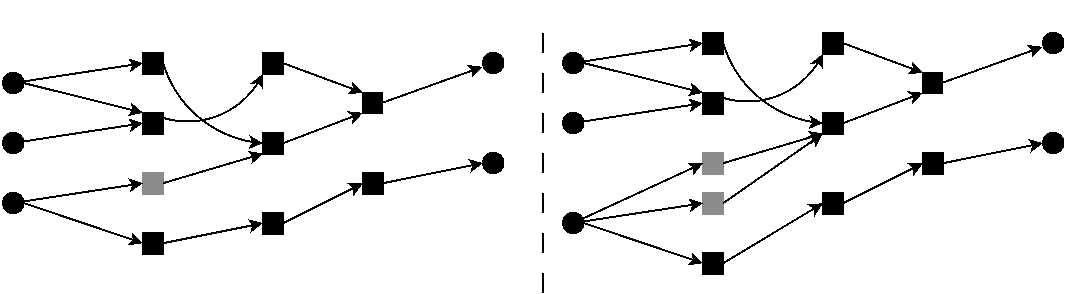
\includegraphics[width=1.0\textwidth]{Bilder/sps_parallel_normal.png}
\caption{Left: An example for an SPS displayed as a directed acyclic graph. Right: Same SPS with introduced parallelity in one operator, marked gray for visibility. Circles are input/outputs, squares are operators, arrows are streams.}
\label{fig:growth_realtime_data}
\end{figure}


\section{Self-Adaptive Systems}
This subchapter should explain what self-adaptive systems are and how they function.
What kind of self-adaptive systems are around?

\section{MAPE-K Loop}
Explain the MAPE-K Loop as it is a valuable basis for many different approaches in adaptive systems


\chapter{Approaches for Self-Adaptive Architectures in Stream Processing}
Explain that this chapter showcases a few select strategies, which are then elaborated on further in the subchapters
Question: Even more approaches? e.g. Master-Slave attern or Coordinated Control pattern (Both MAPE based)?

\section{Dhalion}
Quick Introduction to Dhalion, this chapter will deal with the Dhalion paper.
\subsection{An Outline of Heron}
Small outline of Heron, as Dhalion is built on top of Twitter's Heron.
\subsection{Dhalion's Architecture}
Explanation of Dhalion's Architecture
\subsection{Evaluation of Dhalion}
Present the paper's findings and evaluations of the Dhalion System.

\section{Hierarchical Control Architectures}
Quick Introduction to hierarchical control architectures, this chapter deals with the Cardellini
paper (An example for such an architecture)
\subsection{Elastic and Distributed DSP Framework}
Explanation of the EDF Architecture, their approaches
\subsection{Possible Solutions for Controlling the Adaptation of Data Stream Processing Operators}

\subsection{Evaluation of EDF}
